\chapter{Experimental phase: mechanical properties and performance of corroded reinforcing steel}
\label{chap-three}

Corrosion is the main aging condition that affects structures, therfore, the success of this study relies on the most accurate representation of the corrosion process. As mentioned in Chapter 2 previous studies developed accelerated corrosion specimens with high current densities and did not account for the passivation of the reinforcing steel. Therefore, a main component of this study is to obtain reliable mechanical properties of the corroded reinforcing steel. To achieve this the experimental process is divided in to three main processes, (1) generate the passive layer in rebar specimens, (2) depassivate and corrode the rebar specimens (3) obtain the mechanical properties of the reinforcing steel by performing tension tests and buckled bar tension tests. It is expected that this careful process will mimic as best as possible the real aging conditions of rebars inside the concrete mix environment. This chapter outlines the rebar preparation, experimental setup, instrumentation, and expected results.
%The experimental portion of this research program consists of a total of 54 buckled bar tension tests using the method proposed by Barcley et al \cite{Barcley2019}.The experimental phase of this research aims at studtying the effects of depassivation in the modified mechanical properties of corroded grade 80 reinforcing steel, and the modification on the bending strain in corroded buckled bars. 

\section{Proposed experimental campaign}

It is known that the steel inside concrete generates a protective film due to the alkaline environment generated by the cement paste. The most common form of corrosion occurs via chloride attacks. During a chloride attack, the chloride in salts contacts the surface of the steel, this initiates the elimination of the protective film in a process known as depassivation. The proposed experimental campaign aims at simulating the process of corrosion as it would occur in a rebar embedded in concrete. The experiment process is outlined here:

\begin{enumerate}
	\item Passivation of the reinforcing steel
	\item Accelerated corrosion  of reinforcing steel
	\item Tension tests
	\item Buckled bar tension (BBT) test
\end{enumerate}

\textbf{Passivation of the reinforcing steel}

In order to simulate the conditions of rebars embedded in concrete, it is necessary to generate the passive layer on the surface of the reinforcing steel. There are two ways of generating the passive layer on the reinforcing steel, (1) embed rebars in concrete and wait for the passive layer to generate, (2) submerge the reinforcing steel in a synthetic pore solution that mimics the cement paste environment. The second option is more suited for material testing since it does not involve any form of demolishing. Ghods et al \cite{Ghods2010} developed different ten pore solutions to generate the passive film on the reinforcing steel surface. It is known that the cement paste has ions of $Ca^{+2}$, $Na^{+}$, $K^{+}$, and $(SO_{4})^{+}$. Therefore out of the ten pore solutions proposed by Ghods et al, five had this ions. Further, the authors presented a comparison on the quality of the passive fil, the film that was shown to have the best quality while having all the ions was selected for this study. The pore solution that is going to be deployed has the following concentrations:

\begin{itemize}
	\item Saturated calcium hydroxide $Ca(OH)_2$
	\item Sodium hydroxide $Na(OH)$ (4.00 g/l)
	\item Potassium hydroxide $(KOH)$ (11.22 g/l)
	\item Calcium sulfate dihydrate $Ca(SO)_4 + 2H_2O$ (13.77 g/l)
\end{itemize}

Since it is important to mimic real life applications, the rebars will be placed in the pore solution as received without any special surface preparation in the area of study. It has been shown that any form of special surface preparation affects the quality of the passive layer . Ghods et al showed that it takes a minimum of 8 to 13 days to generate the passive layer \cite{Ghods2009}, therefore the rebars will be placed in the pore solution for a minimum of 13 days. Figure \fref{fig:RebarPassivation} shows. 

In addition, it is necessary to protect the areas of the rebar that are going to function as grips for the rebars during the tension and BBT tests. Therefore the ends of the rebars will be protected with three different layers of protection. First a layer of two-part epoxy is placed, then a layer of electroplater tape and the third and final layer is shrink tube. This three layers ensure minimal corrosion in the grip areas of the rebar. Figures \fref{fig:RebarSpecimenGeomtry} and \fref{fig:RebarEndsProtection} show the specimen geometry and the preparation of the ends of the rebars.

\begin{figure}[htbp]
	\centering
	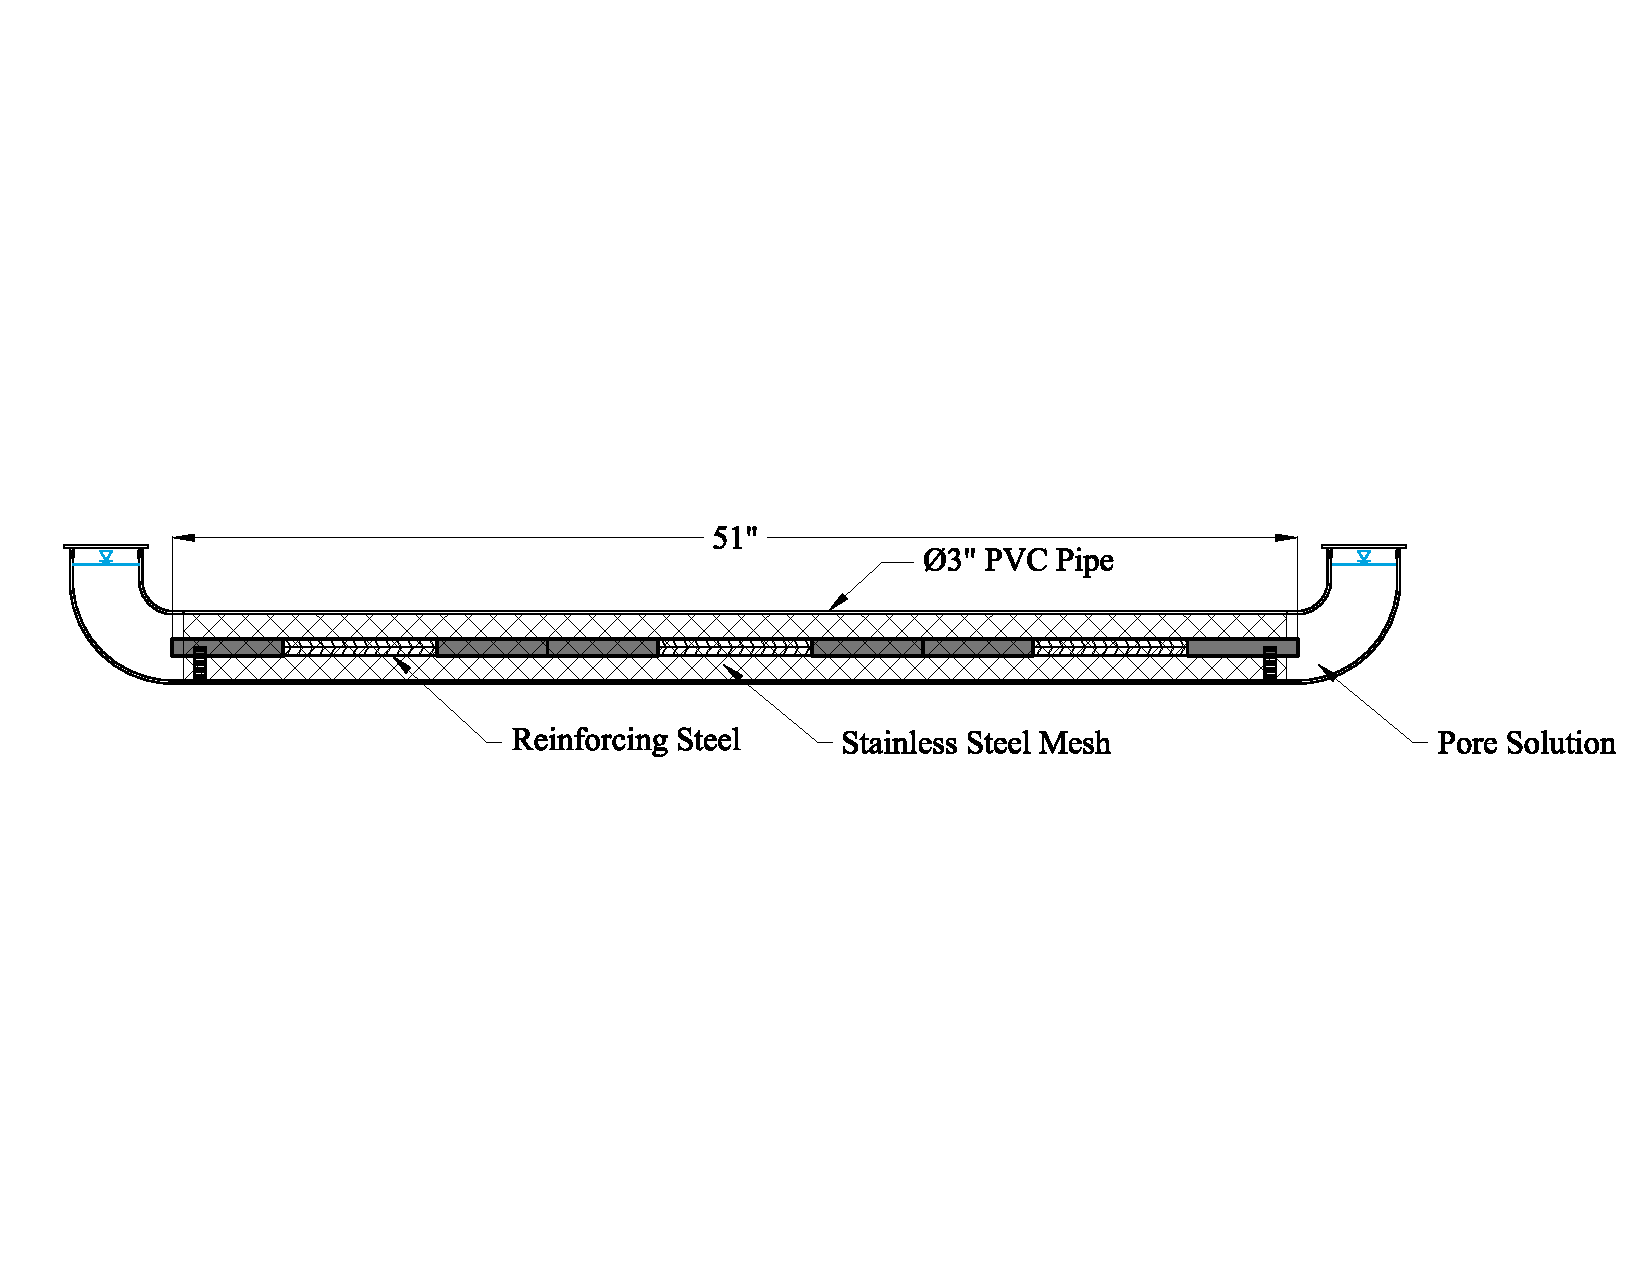
\includegraphics[width=1.0\textwidth]{Chapter-3/figs/AnodicPolarization_01}
	\caption{Rebars Passivation Process in Calcium Hydroxyde Pore Solution}
	\label{fig:RebarPassivation}
\end{figure}

\begin{figure}[htbp]
	\centering
	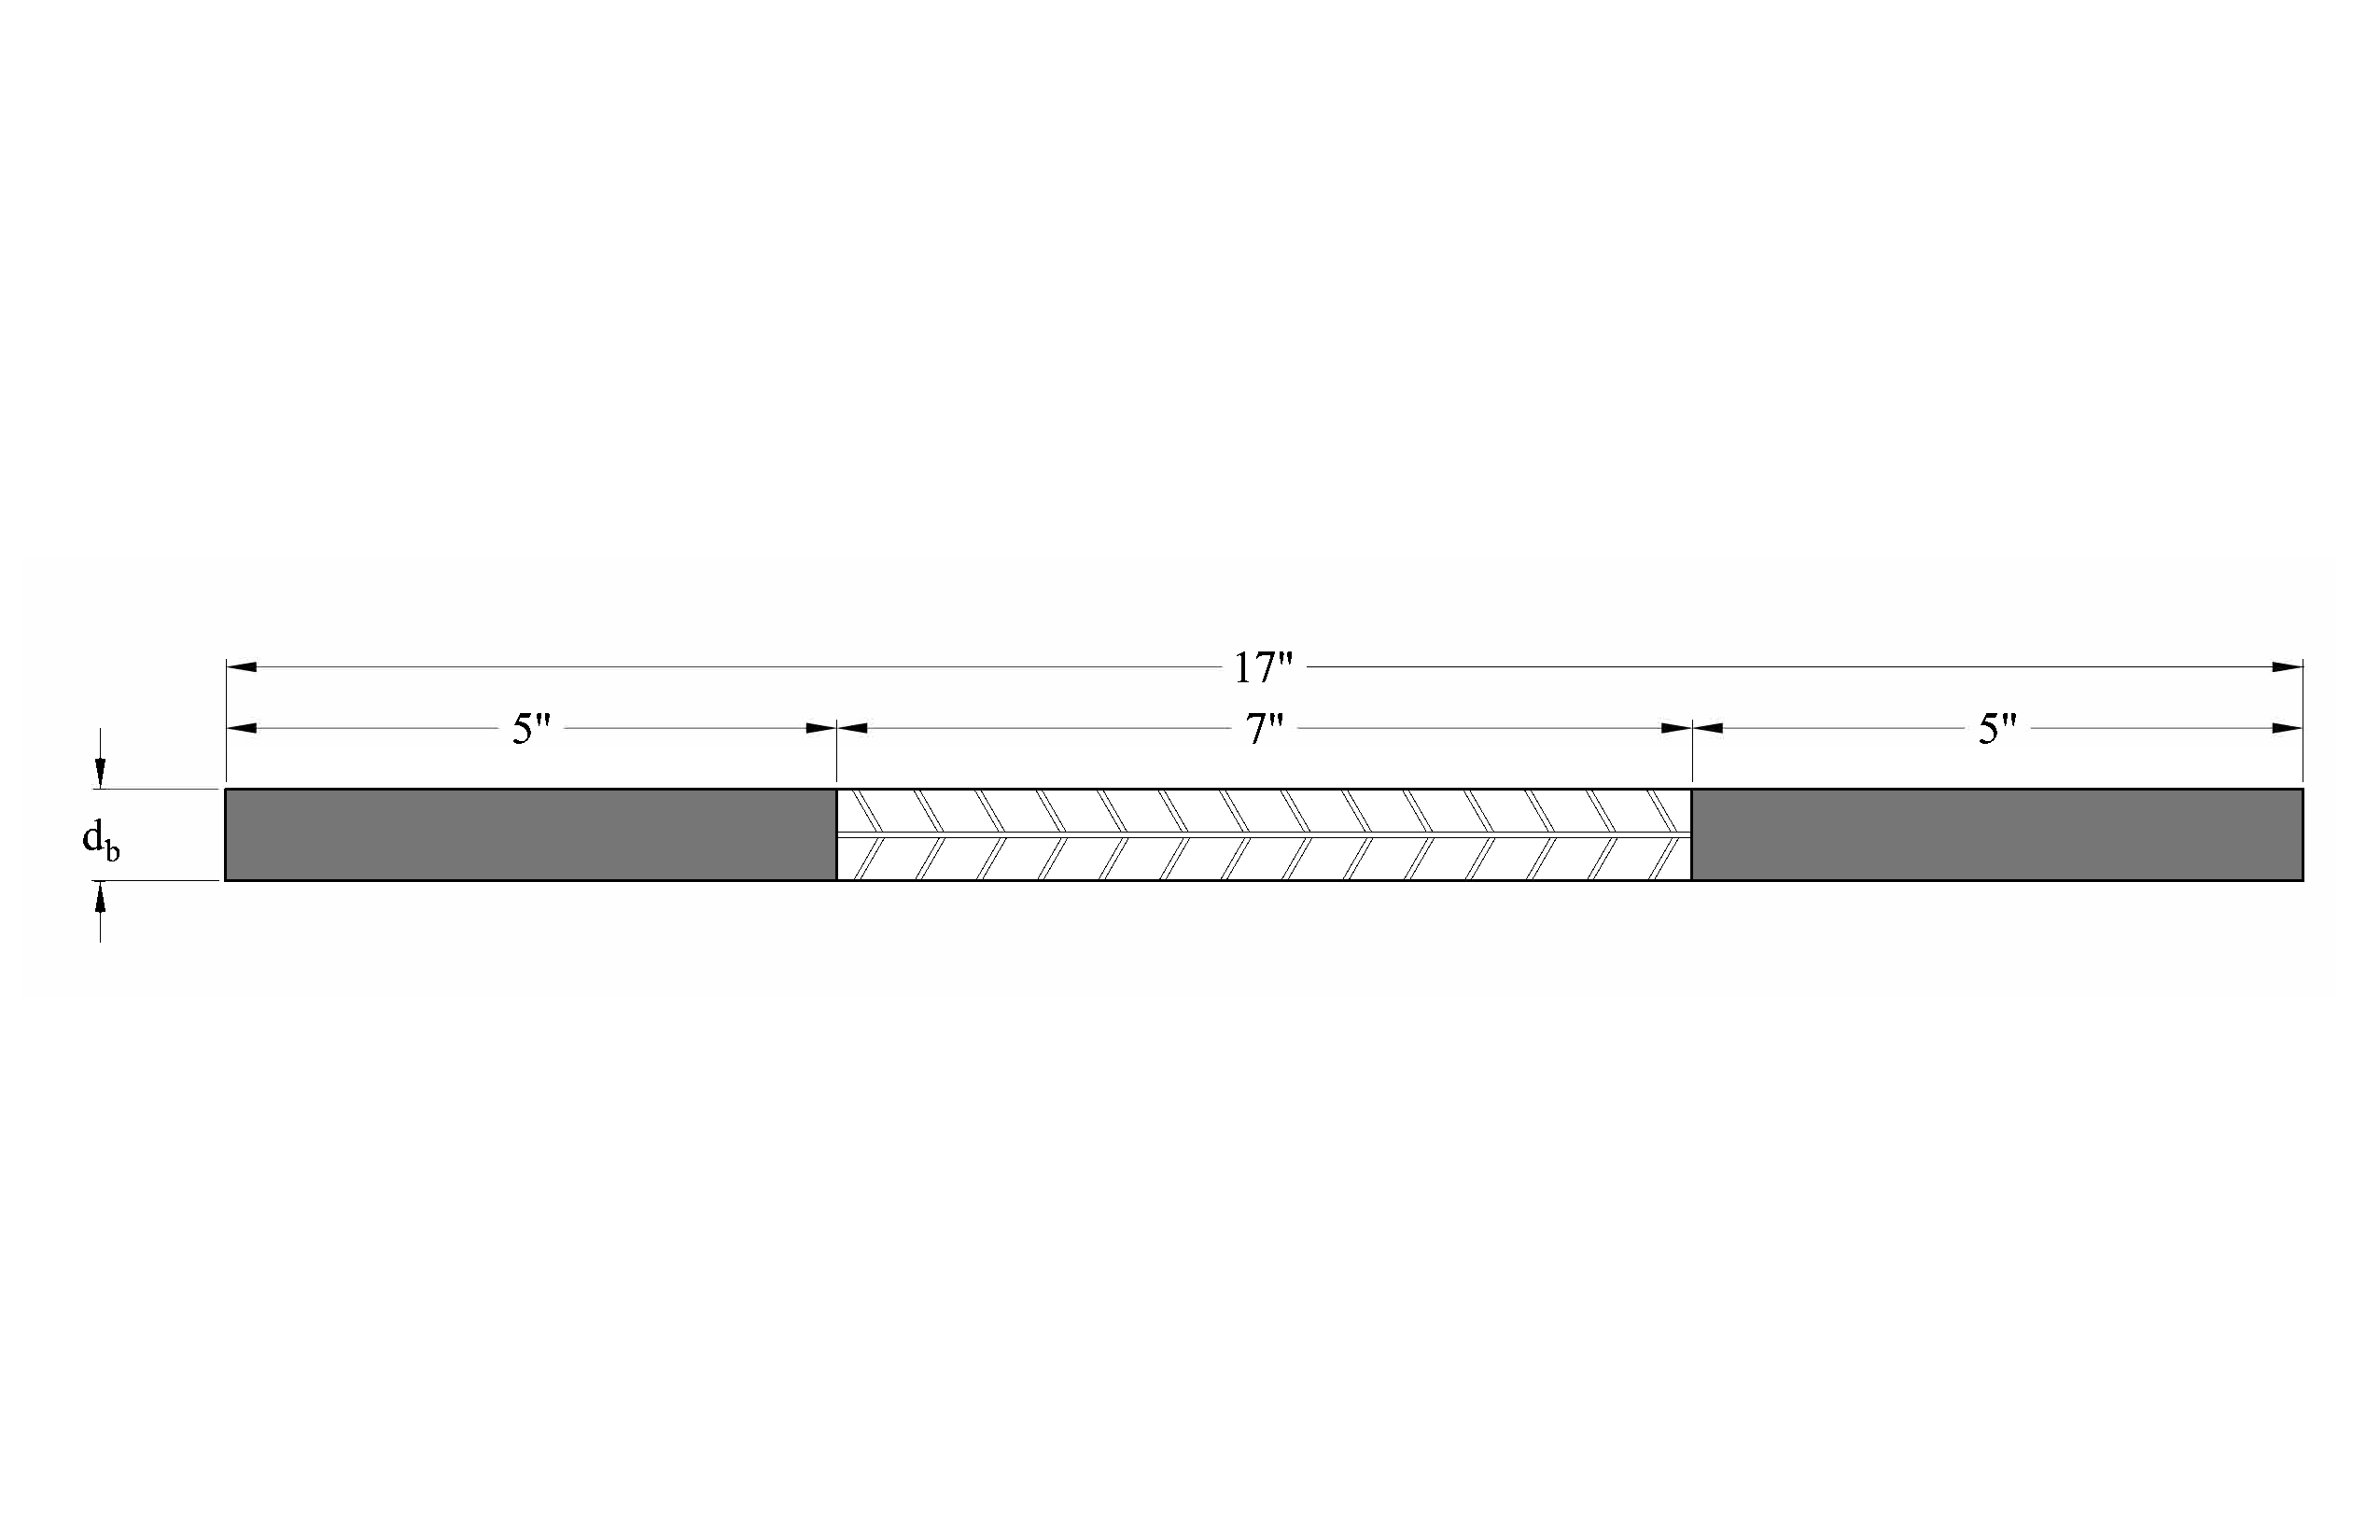
\includegraphics[width=0.9\textwidth]{Chapter-3/figs/RebarSamples}
	\caption{Rebar Specimen Geometry}
	\label{fig:RebarSpecimenGeomtry}
\end{figure}

\begin{figure}[htbp]
	\centering
	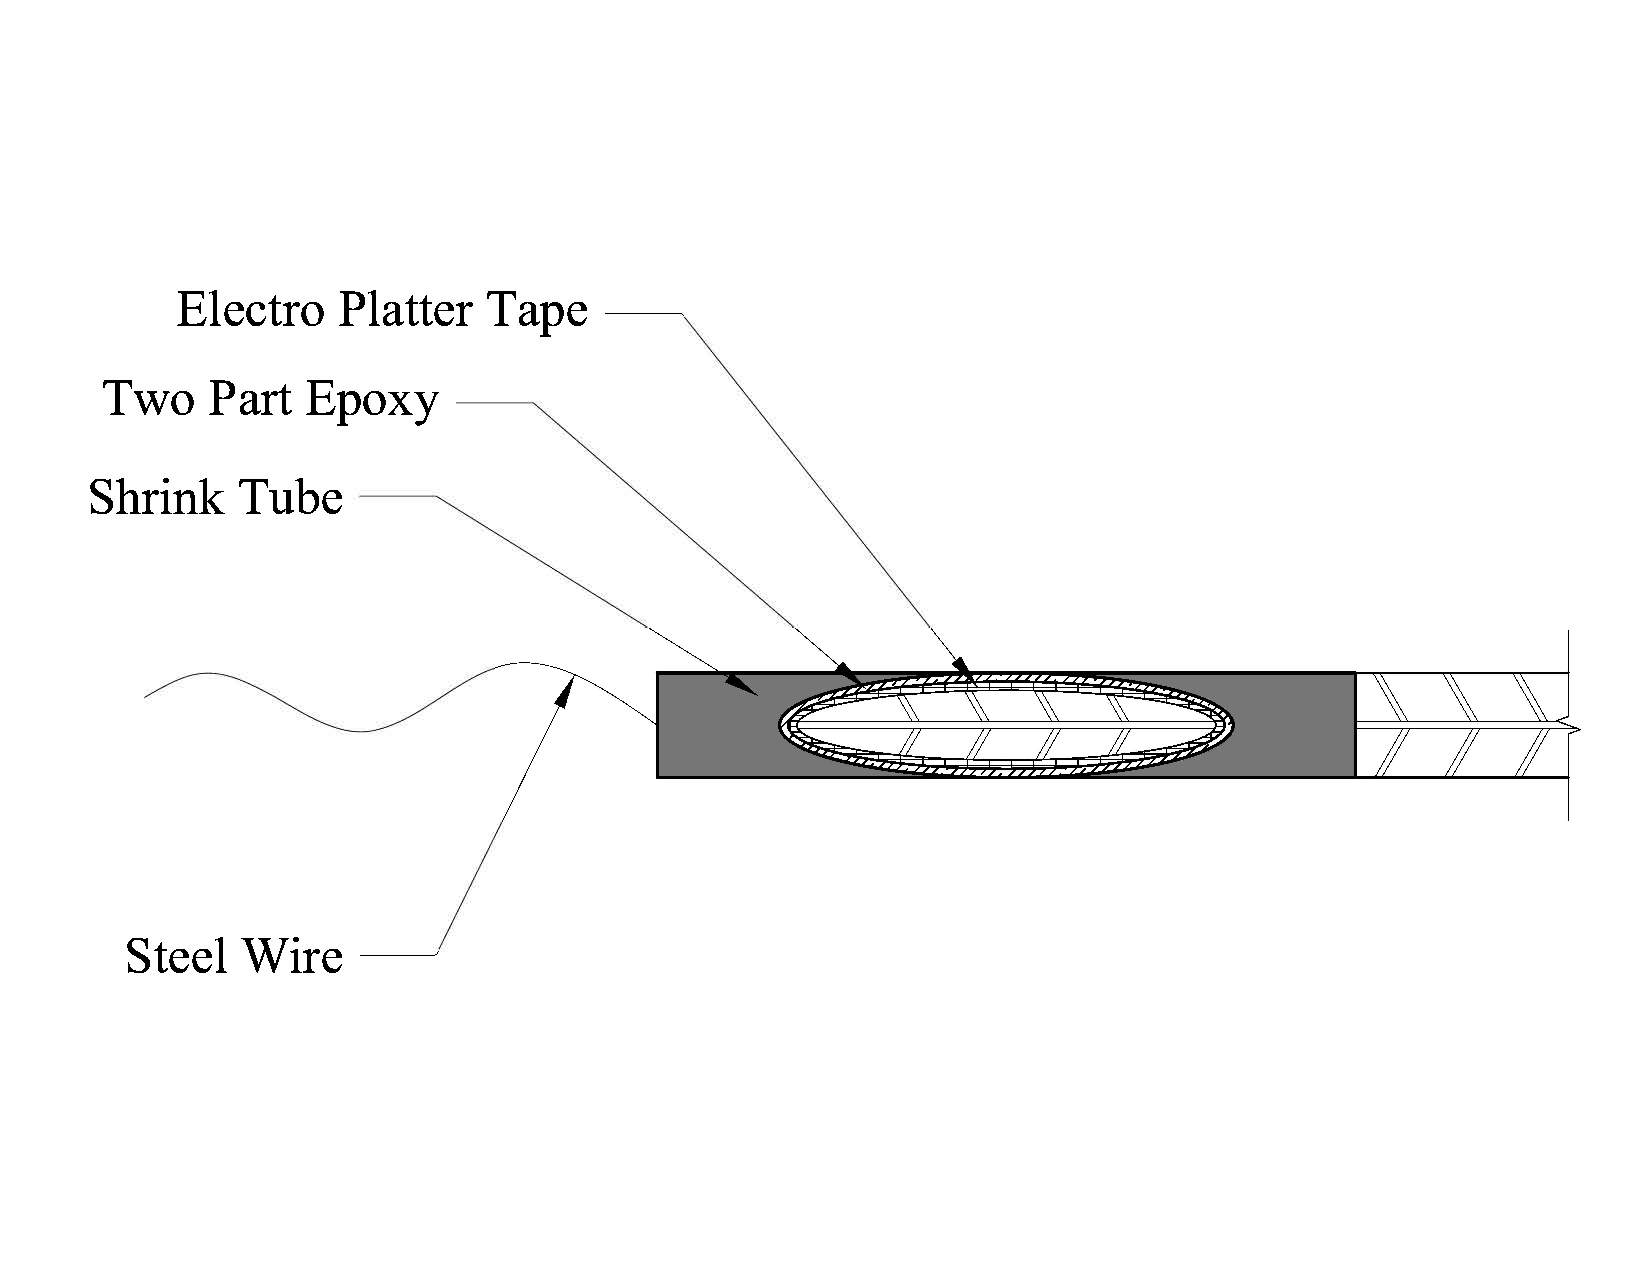
\includegraphics[width=0.9\textwidth]{Chapter-3/figs/Rebar_Ends}
	\caption{Rebars Ends Protection}
	\label{fig:RebarEndsProtection}
\end{figure}


\textbf{Accelerated corrosion  of reinforcing steel}

The accelerated corrosion will be done by using a galvanic cell. Different studies \cite{Ghods2010} have shown that for rebars with pasive films a concentration of 0.3 Moles of sodium chloride ($NaCl$) will start the depassivation process on the rebars. In the study presented here, the specimens will be subjected to a current of 5mA equivalent to $47\mu A/cm^2$. This current is sustained for a period of time according to Faraday's Law until the desired level of corrosion is reached.

\begin{equation}
	t=\frac{\lambda m_{loss} \eta_{specimen} C_{faraday}}{i M_{specimen}}
	\label{eq.FaradayEq}
\end{equation}

\begin{figure}[htbp]
	\centering
	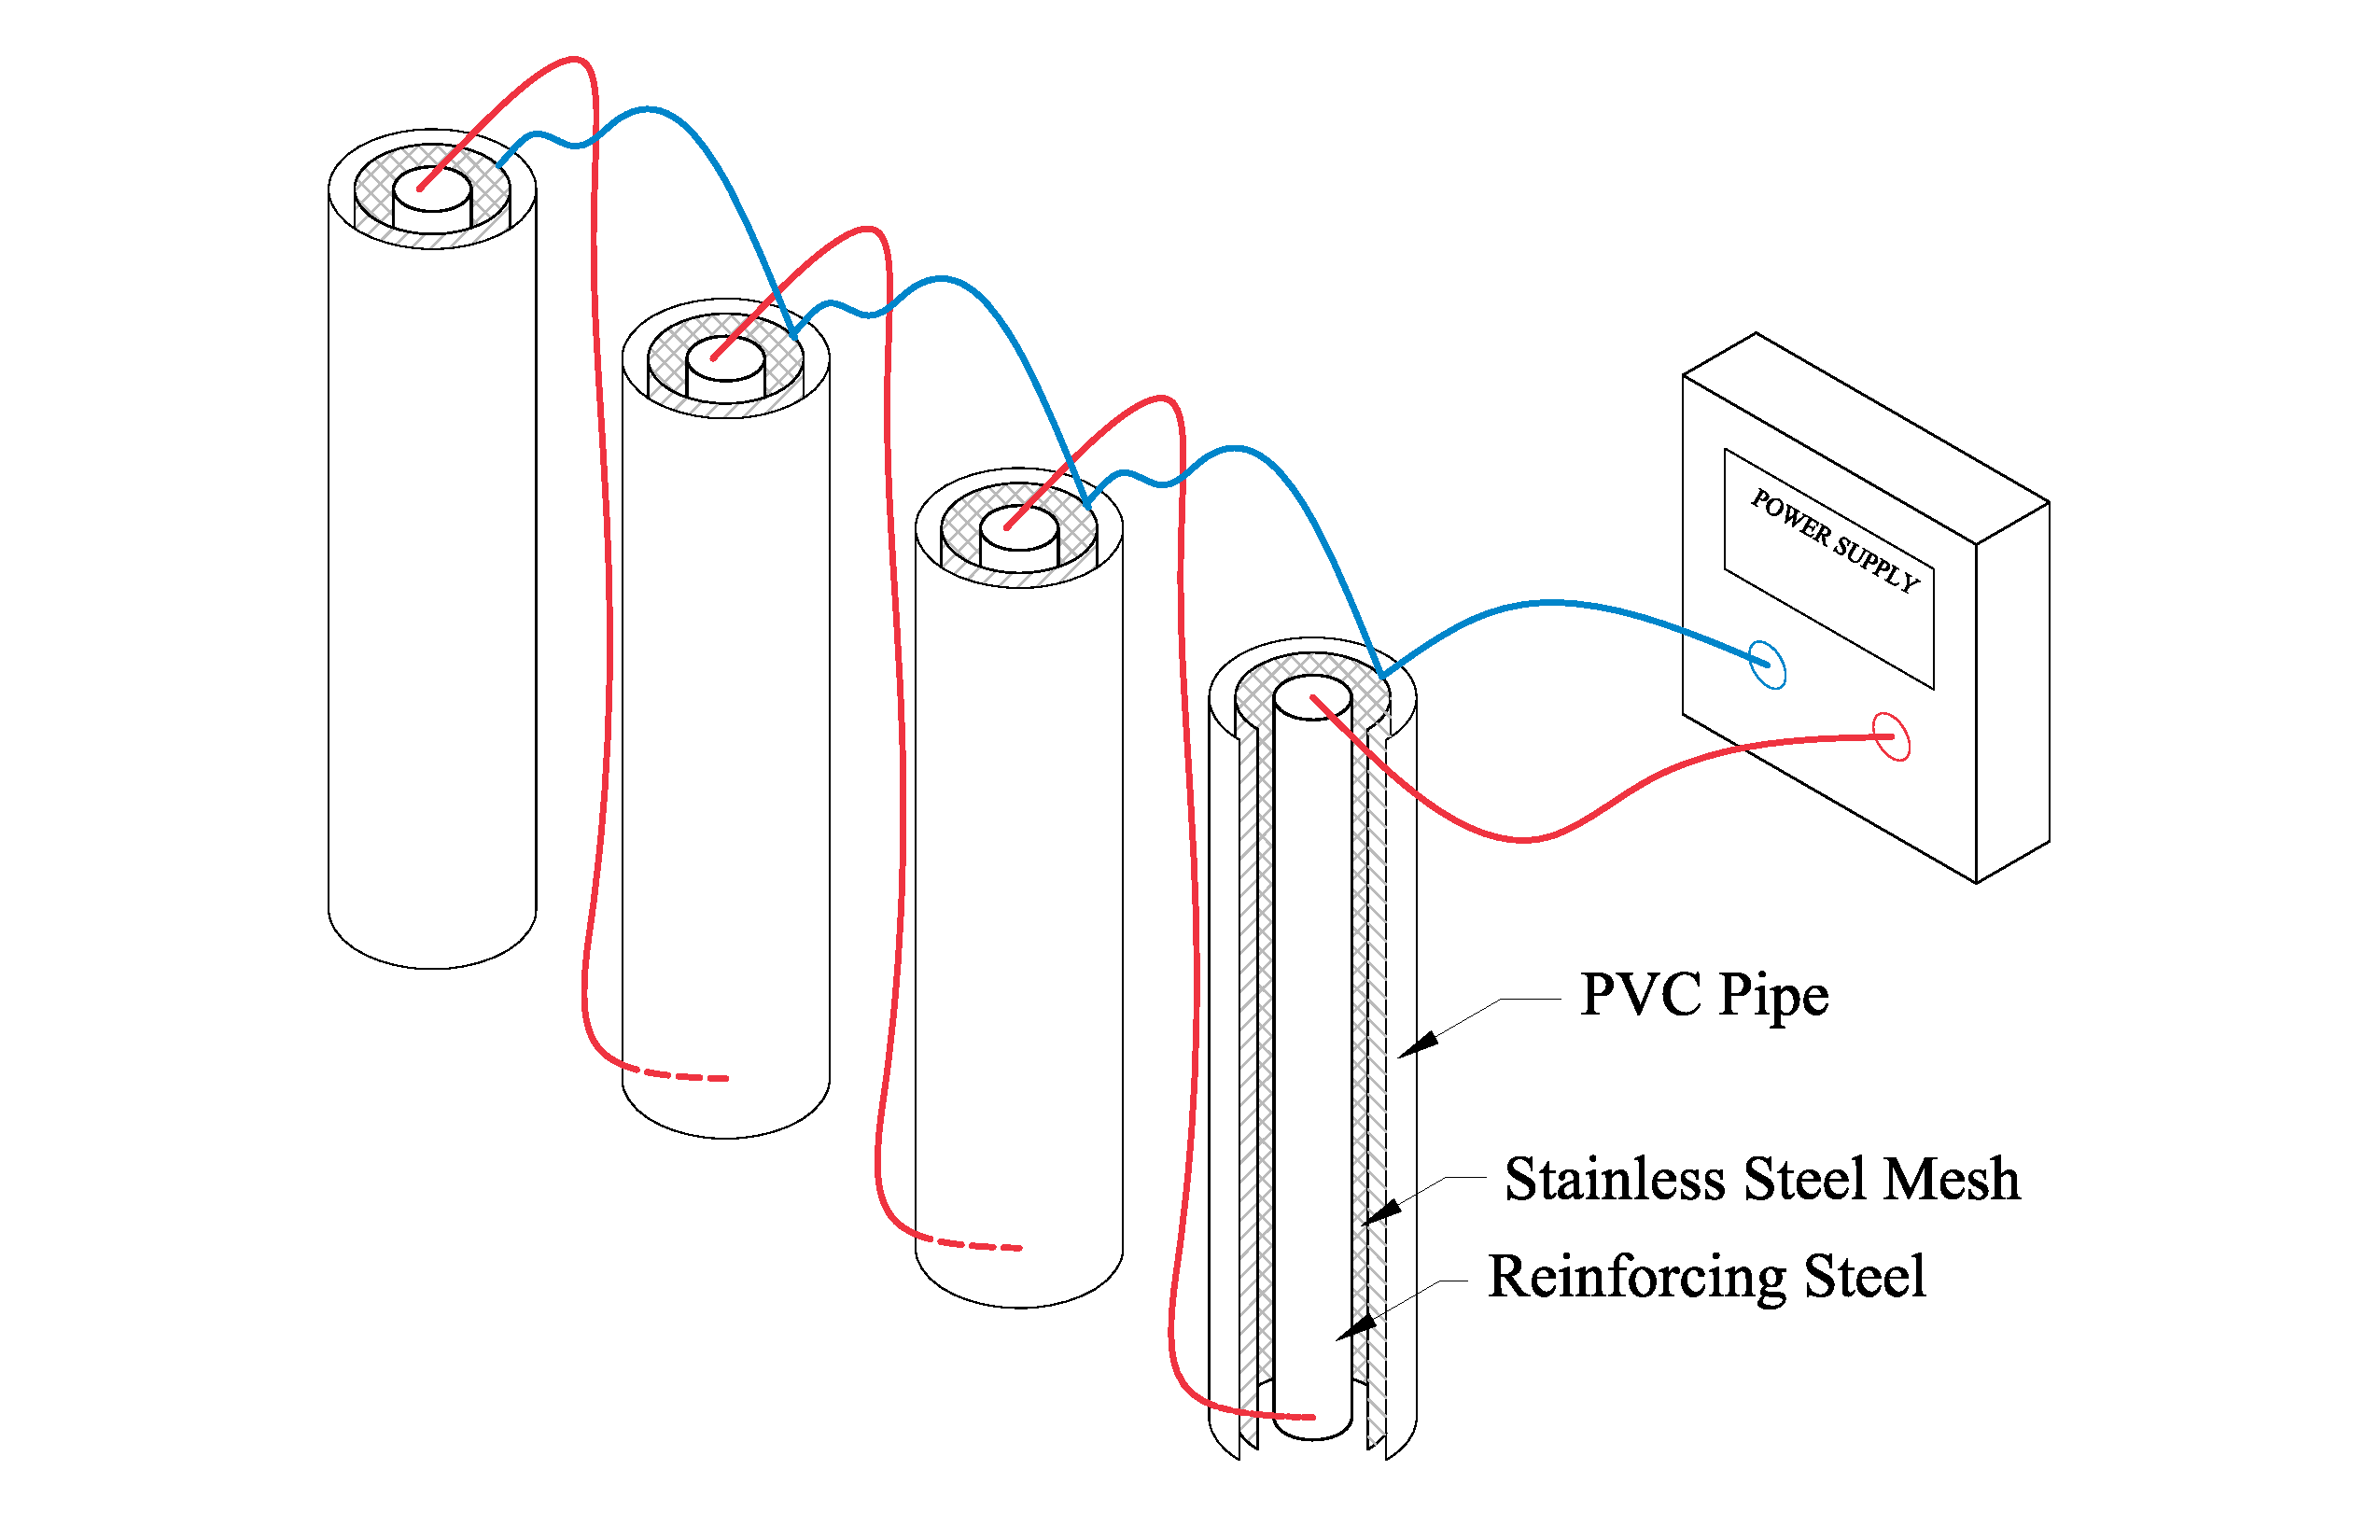
\includegraphics[width=0.9\textwidth]{Chapter-3/figs/AcceleratedCorrosionProcedure}
	\caption{Accelerated corrosion process}
	\label{fig:AcceleratedCorrosion}
\end{figure}

The corrosion levels, the current and the time of application is shown in Table \ref{tab:AcceleratedCorrosionTime}. 

\begin{table}[htbp]
	\caption{Accelerated corrosion times in 3/4" rebar}
	\label{tab:AcceleratedCorrosionTime}
	\centering	
		\begin{tabular}{|l|c|c|}
		\hline
		Corrosion Level (CL) & Mass loss (g)   & time(days)     \\  \hline	
		5\%                  & 1.12            & 9  \\  \hline	
		10\%                 & 2.24            & 18 \\  \hline	
		15\%                 & 3.36            & 27 \\  \hline	
		20\%                 & 4.47            & 36 \\  \hline	
		25\%                 & 5.59            & 45 \\  \hline	
		\end{tabular}
\end{table}
\newpage

\textbf{Tension tests}

A series of tension tests will be performed according to ASTM A370. The main objective of this tests is to evaluate differences in the stress-strain behavior of corroded reinforcing steel. This will determine if there is any reduction in the ductility of steel for this condition.
\newline

\textbf{Buckled bar tension (BBT) test}

One of the limit states that control performance-based design is buckling of reinforcing steel, recent tests have been developed to determine the critical bending strain of buckled reinforcing steel \cite{Barcley2019}. The buckled bar tension (BBT) test simulates bending and tension strain demands on a buckled bar, to determine critical bending strain in buckled rebars. 

Barcley et al \cite{Barcley2019} developed a methodology to calculate local strains on a buckled bar using an LED optical sensor system \cite{NorthernDigitalInc.2020}. The procedure is illustrated in \fref{fig:BBTseq}.

\begin{figure}[htbp]
	\centering
	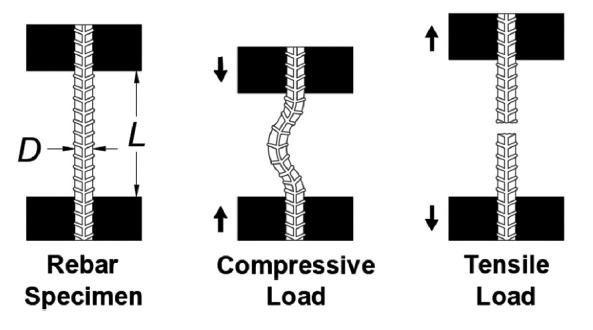
\includegraphics[width=0.7\textwidth]{Chapter-3/figs/BBT_Sequence}
	\caption{BBT Test sequence\cite{Barcley2019}}
	\label{fig:BBTseq}
\end{figure}

The procedure to perform the buckled bar tension test consists of:

\begin{enumerate}
    \item First, place rebar in a univeral testing machine (UTM), and prepare the rebar specimen with LED markers on the surface of the specimen such that the displaced shape of the bar can be measured.
    \item Second, compress the rebar specimen to impose a bending strain of a prescribed level. Barcley et al showed that a fourth order polynomial can be fit to the LED sensors near the buckled region of the bar to obtain the displaced shape ($w$). The bending strain is calculated using solid mechanics principles. Curvature is the second derivative of the displaced shape ($w$) for small displacements is calculated as: 
    \begin{equation}
        \phi=\frac{\frac{d^2w(x)}{dx^2}}{\left[1+\left(\frac{dw(x)}{dx}\right)\right]^\frac{3}{2}}\approx \frac{d^2w(x)}{dx^2}
        \label{eq.CuvatureAprox}
    \end{equation}
    If we assume that the bending is symmetric for the rebar then the strain in the extreme fibers of the rebar is calculated as:
    \begin{equation}
        \varepsilon_{b}=\phi\left(\frac{d_{bl}}{2}\right) 
        \label{eq.BendingStrain}
    \end{equation}    
    Combining equations \eref{eq.CuvatureAprox}, and \eref{eq.BendingStrain} then the bending strain can be expressed as:
    \begin{equation}
        \varepsilon_{b}=\frac{d^2w(x)}{dx^2}\left(\frac{d_{bl}}{2}\right) 
        \label{eq.BendingStrainExpanded}
    \end{equation}
    An example of the calculation of the bending strain is shown in \fref{fig:BBT_Curvature}
    \item Second, Once buckled to the prescribed curvature, the bar is loaded in tension until fracture is observed
    \item Then the process is repeated with a different bar for a different bending strain. After all the tests are performed results from elongation at peak force can be generated as the example shown in \fref{fig:BBT_MaxBendingStrain}. From the results obtained through BBT tests the critical bending strain can be determined. The critical bending strain is defined as the point at which a low elongation under load is obtained. This low elongation results in a brittle fracture of the rebar as shown in \fref{fig:BBT_DuctileBrittle}(b). \fref{fig:BBT_MaxBendingStrain} shows that for bars with rebars the critical bending strain is $\varepsilon_{b}=0.10$ for grade 80 ksi steel.
\end{enumerate}

\begin{figure}[htbp]
    \centering
    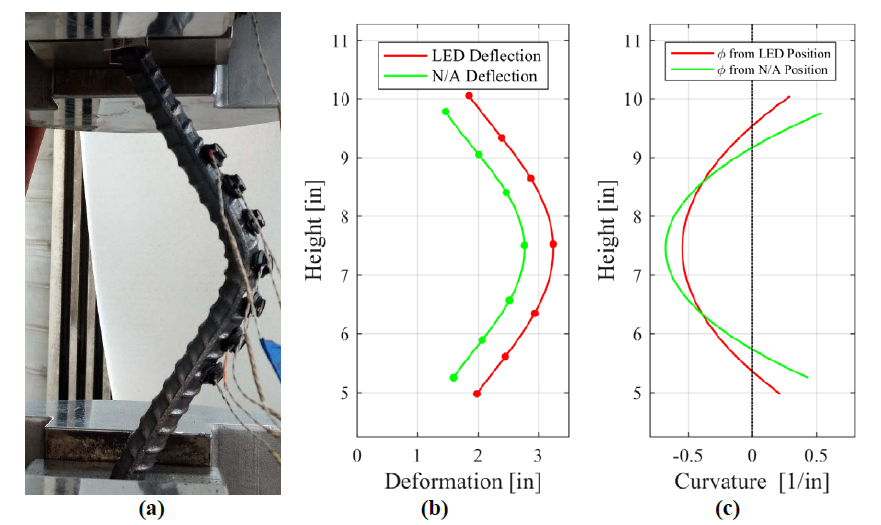
\includegraphics[width=1\textwidth]{Chapter-3/figs/BBT_Curvature}
    \caption{a) Picture of buckled bar; (b) Position of optical markers and adjustment to neutral axis; (c) Calculation of curvature \cite{Barcley2018}}
    \label{fig:BBT_Curvature}
\end{figure}
\begin{figure}
    \centering
    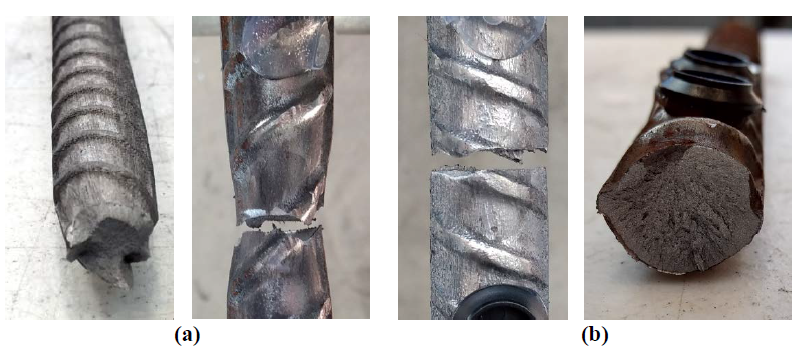
\includegraphics[width=1\textwidth]{Chapter-3/figs/BBT_Ductile_vs_Brittle}
    \caption{(a)Ductile rebar fracture; (b) Brittle rebar fracture \cite{Barcley2018}}
    \label{fig:BBT_DuctileBrittle}
\end{figure}
\begin{figure}[htbp]
    \centering
    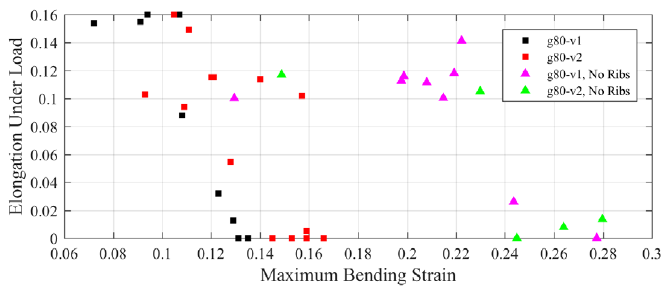
\includegraphics[width=0.8\textwidth]{Chapter-3/figs/BBT_MaxBendignStrain}
    \caption{BBT results for rebars with and without ribs \cite{Barcley2018}}
    \label{fig:BBT_MaxBendingStrain}
\end{figure}

The BBT test is proposed for different levels of corrosion such that any changes on the behavior are studied and incorporated in the analytical model. The proposed test matrix is shown in Table \ref{tab:Test Matrix}. It must be noted that in each corrosion level for the BBT tests, each experiment will correspond to a different prescribes bending strain. The selection for each prescribed bending strains consists in 1) Start with the maximum bending strain determined in previous research to be around $\varepsilon=0.10$ as shown in \fref{fig:BBT_MaxBendingStrain}, 2)if brittle fracture is observed the next test will be at a lower bending strain for example $\varepsilon=0.08$, 3)otherwise higher strains such as $\varepsilon=0.12$ will be evaluated, this is repeated for each corrosion level. It is expected that six tests per corrosion level will be sufficient however, more tests will be performed if necessary. The results obtained will be compared to those of a pristine condition rebar which corresponds to a corrosion level of $CL=0\%$

% Please add the following required packages to your document preamble:
% \usepackage{multirow}
% \usepackage[table,xcdraw]{xcolor}
% If you use beamer only pass "xcolor=table" option, i.e. \documentclass[xcolor=table]{beamer}
\begin{table}[htb]
	\caption{Corroded Rebar Test Matrix}
	\label{tab:Test Matrix}
	\centering	
	\begin{tabular}{|c|c|c|c|}
	\hline
	\multicolumn{4}{|c|}{\cellcolor[HTML]{CC0000}{\color[HTML]{FFFFFF} Corroded rebar test matrix}}                                               \\ \hline
	\multicolumn{1}{|l|}{Test}     & \multicolumn{1}{l|}{Diameter of bar} & \multicolumn{1}{l|}{CL (\%)} & \multicolumn{1}{l|}{Number of Tests} \\ \hline
	                               &                                      & 0                            & 3                                    \\ \cline{3-4} 
	                               &                                      & 5                            & 3                                    \\ \cline{3-4} 
	                               &                                      & 10                           & 3                                    \\ \cline{3-4} 
	                               &                                      & 15                           & 3                                    \\ \cline{3-4} 
	                               &                                      & 20                           & 3                                    \\ \cline{3-4} 
	\multirow{-6}{*}{Tension test} & \multirow{-6}{*}{\#6}                & 25                           & 3                                    \\ \hline
	                               &                                      & 0                            & 6                                    \\ \cline{3-4} 
	                               &                                      & 5                            & 6                                    \\ \cline{3-4} 
	                               &                                      & 10                           & 6                                    \\ \cline{3-4} 
	                               &                                      & 15                           & 6                                    \\ \cline{3-4} 
	                               &                                      & 20                           & 6                                    \\ \cline{3-4} 
	\multirow{-6}{*}{BBT test}     & \multirow{-6}{*}{\#6}                & 25                           & 6                                    \\ \hline
	\end{tabular}
\end{table}

\section{Expected outcomes from experimental phase}

The results from the tension tests will help to establish if the depassivation process in the corroded rebars has an effect on the measured stress-strain relationship of steel as has been observed in previous research which did not considered the depassivation process \cite{Meda2014},\cite{Yuan2017a},\cite{Du2005}. Similarly the results from the BBT tests will show any changes in the critical bending strain of rebars as they corrode. The critical bending train impacts the bar fracture limit state. In the case of corroded rebars it is expected that the critical bending strain will be modified by changes in the mechanical properties of steel due to corrosion, and effects of concentrated corrosion along the surface of the rebars. These two factors we hypothesize will induce fracture at a lower bending strain than those observed in pristine conditions rebars\cite{Barcley2019}.

The results obtained from the experiment will also be used to define the bar fracture limit state for RC columns. Research currently being developed at NC State will provide models that allows to establish bar fracture tensile strain while considering different parameters such as transverse steel spacing, axial load ratio, strength of the concrete to mention a few. The model will be similar to that presented by Barcley et al \cite{Barcley2018} shown in EQ. This model could then be implemented in the analytical model presented in \ref{chap-four}. If fracture occurs at a lower strain in corroded rebars, this implies that the corroded RC columns are prone to reach the fracture bar limit state at a much lower displacement than in a pristine RC column.

Future studies will verify the application of the results found in this research to perform full scale corroded RC column that consider the effect of depassivation in the cyclic behavior of such columns.